\chapter{Considerações Gerais}
\label{cap:02}

Texto das considerações gerais, dividido em subseções.

Este é um exemplo de como usar figuras. Referência cruzada: Figura~\ref{fig:exemplo}

\FloatBarrier
\begin{figure}[!htbp]
	\centering
	\caption{Exemplo de figura}
	%scale redimensiona a figura.
	%1.5 = 150% do tamanho original
	%1 = 100% do tamanho original
	%0.20 = 20% do tamanho original
	
\includegraphics[scale=0.4]{imagens/exemploFigura}
	\\\textbf{Fonte:} Elaborada pelo autor
	\label{fig:exemplo}
\end{figure}
\FloatBarrier


Este é um exemplo de como usar tabelas. Referência cruzada: Tabela~\ref{tab:exemplo}

\FloatBarrier
\begin{table}[!htbp]
	\centering
	\caption{Exemplo de tabela de 2 colunas}
	\begin{tabular}{ c | c }
		\hline
		\textbf{Coluna 1} & \textbf{Coluna 2} \\ \hline
		Dado 1a           & Dado 2a           \\ \hline
		Dado 1b           & Dado 2b           \\ \hline
		Dado 1c           & Dado 2c           \\ \hline
		Dado 1d           & Dado 2d           \\ \hline
	\end{tabular}
	\\ \vspace{0.2cm}
	\textbf{Fonte:} Elaborada pelo autor
	\label{tab:exemplo}
\end{table}
\FloatBarrier


Este é um exemplo de como usar quadros. Referência cruzada: Quadro~\ref{qua:exemplo}

\FloatBarrier
\begin{quadro}[!htbp]
	\centering
	\caption{Exemplo de quadro}
	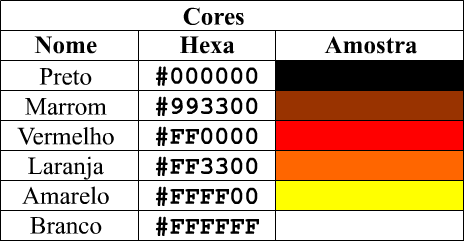
\includegraphics[scale=.7]{imagens/exemploQuadro}
	\\\textbf{Fonte:} Elaborada pelo autor
	\label{qua:exemplo}
\end{quadro}
\FloatBarrier


Este é um exemplo de como usar equações. Referência cruzada: Equação~\ref{eq:exemplo}

\begin{equation}
\sum_{i=1}^{n} i = \frac{n(n+1)}{2}
\label{eq:exemplo}
\end{equation}


Exemplo de inserção de lista de código fonte:

\lstinputlisting[language=Java]{fontes/ClasseExemplo.java} 



Este é um exemplo de como inserir texto sem formatação (ambiente verbatim):

\begin{verbatim}
Texto sem formatação, como espaçamento igual.
\end{verbatim}


Exemplo de lista de itens:

\begin{itemize}
	\item \textbf{Item 1:} texto...;
	\item \textbf{Item 2:} texto...;
	\begin{itemize}
		\item \textbf{Subitem:} texto...;
		\item \textbf{Subitem:} texto...;
		\item \textbf{Subitem:} texto...;
	\end{itemize}
	\item \textbf{Item 3:} texto...;
	\item \textbf{Item n:} texto....
\end{itemize}


Exemplo de lista numerada:

\begin{enumerate}
	\item \textbf{Item:} texto...;
	\item \textbf{Item:} texto...;
	\begin{enumerate}
		\item \textbf{Subitem:} texto...;
		\item \textbf{Subitem:} texto...;
		\item \textbf{Subitem:} texto...;
	\end{enumerate}
	\item \textbf{Item:} texto...;
	\item \textbf{Item:} texto....
\end{enumerate}


Exemplos de comandos para texto e referências:

\begin{itemize}
	\item Para iniciar um novo parágrafo, basta deixar uma linha em branco no código fonte;
	\item Não force o compilador a pular mais de uma linha, pois terá influência negativa na composição do documento;
	\item Sempre deixe o \LaTeX\ realizar a formatação de parágrafos e posicionamento de elementos;
	\item Utilização de aspas simples (abertura \verb|`|, fechamento \verb|'|): `Texto entre aspas simples';
	\item Utilização de aspas duplas (abertura \verb|``|, fechamento \verb|''|): ``Texto entre aspas duplas'';
	\item Negrito (comando \verb|\textbf|): \textbf{texto em negrito};
	\item Itálico (comando \verb|\textit|): \textit{texto em itálico};
	\item Sublinhado (comando \verb|\underline|): \underline{texto sublinhado};
	\item Negrito e itálico (usar comandos juntos): \textbf{\textit{texto em negrito e itálico}};
	\item Alterar cor do texto (comando \verb|\textcolor{cor}{texto}|):
	\begin{itemize}
		\item Exemplo \verb|\textcolor{red}{texto}|: \textcolor{red}{texto vermelho};
		\item Exemplo \verb|\textcolor[RGB]{255, 102, 0}|: \textcolor[RGB]{255, 102, 0}{texto laranja};
		\item Exemplo \verb|\textcolor[HTML]{006AD7}|: \textcolor[HTML]{006AD7}{texto azul};
	\end{itemize}
	\item Ambiente matemático inline (comando \verb|$ expressão $|): $s = x^2-2x +1$;
	\item Referência normal (comando \verb|\cite|):
	\begin{itemize}
		\item \cite{Agaisse1995};
		\item \cite{Abedi2014};
		\item \cite{BtNomenclature2016};
	\end{itemize}
	\item Referência normal com mais de uma obra (comando \verb|\cite|):
	\begin{itemize}
		\item \cite{Abedi2014, Agaisse1995};
        \item \cite{AgapitoTenfen2014, BtNomenclature2016, Nelson2014};
	\end{itemize}
	\item Referência nome e ano (comando \verb|\citeauthorandyear|):
	\begin{itemize}
		\item \citeauthorandyear{Agaisse1995};
		\item \citeauthorandyear{Abedi2014};
		\item \citeauthorandyear{BtNomenclature2016};
	\end{itemize}
\end{itemize}


Exemplo 1 de citação direta:

\begin{citacao}
	Os 20 aminoácidos usualmente encontrados como resíduos em proteínas contém um grupo $\alpha$-carboxil, um grupo $\alpha$-amino e um grupo R distinto substituído no átomo de carbono $\alpha$. O átomo de carbono $\alpha$ de todos os aminoácidos, com exceção da glicina, é assimétrico e, portanto, os aminoácidos podem existir em pelo menos duas formas estereoisoméricas. Somente os estereoisômeros L, com uma configuração relacionada à configuração absoluta da molécula de referência L-gliceraldeído, são encontrados em proteínas \cite[p. 81]{Nelson2014}.
\end{citacao}

Exemplo 2 de citação direta:

\begin{citacao}
	\textit{These various insecticidal proteins are synthesized during the stationary phase and accumulate in the mother cell as a crystal inclusion which can account for up to 25\% of the dry weight of the sporulated cells. The amount of crystal protein produced by a B. thuringiensis culture in laboratory conditions (about 0.5 mg of protein per ml) and the size of the crystals (24) indicate that each cell has to synthesize $10^6$ to $2 \times 10^6$ $\delta$-endotoxin molecules during the stationary phase to form a crystal} \cite[p. 1]{Agaisse1995}.
\end{citacao}

Exemplo de nota de rodapé\footnote{Essa é uma nota de rodapé!}.


\section{Trabalhos Correlatos}

Pesquise e descreva no mínimo três trabalhos correlatos ao seu.

Trabalhos relacionados a tetris.

Trabalhos relacionados a Game Design.

Trabalhos relacionados a Arquitetura de jogos.

Trabalhos relacionados a Jogos em gerais.

\section{O que é um Jogo?}
Criar e participar de jogos desde os períodos mais
antigos da história é um impulso básico do Homo 
sapiens. Desde nossos ancestrais mais remotos,
passando por civilizações como os gregos e os 
romanos, até os dias atuais, sempre existiram 
sistemas e práticas voltados ao ato de jogar, 
tendo como finalidade o entretenimento, a competição
e a educação \cite{egenfeldt2020understanding}.

Um jogo pode ser considerado uma atividade de ocupação
voluntária, realizada dentro de certas limitações de tempo
e espaço, seguindo regras determinadas e obrigatórias, 
com o objetivo de alcançar uma meta específica, gerando
sensações de tensão, desafio e alegria \cite{vasques2025jogar}.

O primeiro jogo eletrônico da história foi lançado em 1958,
chamado Tennis for Two. Seu objetivo era simular uma quadra
de tênis 2D e ele foi criado exclusivamente para entretenimento,
permitindo que duas pessoas jogassem presencialmente. Com o
passar dos anos, os jogos foram evoluindo e passaram a ser exibidos
em telas de televisão e computadores, com imagens mais dinâmicas, 
recursos sonoros aprimorados e maior exigência de habilidade e 
aprendizado por parte dos jogadores.

No livro "Understanding Video Games: The Essential Introduction"
\cite{egenfeldt2020understanding}, os autores explicam que existem
diversas metodologias de análise do que é jogo, sendo três os principais
elementos:

\begin{enumerate}
	\item \textbf{Regras:} O game design que define a estrutura do jogo;
	\item \textbf{Experiência Humana:} O grau de envolvimento e imersão do jogador;
	\item \textbf{Cultura:}  O contexto no qual o jogo está inserido
\end{enumerate}

Esses três elementos quando juntos em uma aplicação, definem o que é um jogo,
 o game design vai definir as mecânicas e regras em um contexto que se 
 está inserido que vai auxiliar na experiencia humana. 

De acordo com Paul Schuytema, no livro "Design de Games — Uma Abordagem
Prática" \cite{schuytema2008design}, um jogo eletrônico é uma forma de 
entretenimento composta por atividades, funções e ações realizadas por 
um jogador, limitado por regras dentro de um universo definido, que resultam 
em uma condição final. O universo e as regras têm a função de dar contexto às 
ações do jogador, além de criar desafios e conflitos.
As decisões e ações do jogador fazem parte do processo que compõe o jogo, 
mas o fator mais importante não é apenas chegar ao final, e sim a experiência
e o envolvimento durante o percurso.



Com base nas definições apresentadas, pode-se considerar que um jogo é
algo criado pelo ser humano, composto por um conjunto de regras e
limitações que estabelecem um desafio e um objetivo específico a ser 
alcançado.
No caso de um jogo eletrônico, a definição é similar, mas com a adição 
de que o game design precisa ser bem estruturado, com elementos para 
que os jogadores se envolvam para a chegada do objetivo, 
tornando a experiência de jogar satisfatória, não apenas pela 
conquista do objetivo final, mas por todo o processo.

\section{Tipos de Jogos não Digitais} %será que eu mudo pra TIpos de jogos Tradicionais??

	\subsection{Jogos de Cartas}
	A categoria de jogos de cartas são aquelas no qual há a interação entre os jogadores através de um baralho de cartas,
	são jogos que requerem uma estratégia para serem jogadas, em torno da análise combinatoria das cartas visiveis aos jogadores ("na mesa")
	e das cartas que está nas mãos dos jogadores. Em muitos jogos de cartas pode ter a interação e comunicação entre jogadores, permitindo o blefe, por exemplo o poker \cite{lucchese2009conceituaccao}
	%adicionar depois uma imagem de jogo de carta, tipo o poker
\FloatBarrier
\begin{figure}[!htbp]
	\centering
	\caption{Exemplo de figura}
	%scale redimensiona a figura.
	%1.5 = 150% do tamanho original
	%1 = 100% do tamanho original
	%0.20 = 20% do tamanho original
	
\includegraphics[scale=0.4]{imagens/exemploFigura}
	\\\textbf{Fonte:} Elaborada pelo autor
	\label{fig:exemplo}
\end{figure}
\FloatBarrier
	\subsection{Jogos de Tabuleiro}
	Os jogos de tabuleiro são os que representam fisicamente um plano jogavel e representam também a divisória de setores
	e um conjunto de peças que podem ser movidas nesse plano ao longo do decorrer do jogo. Essas peças devem ser associadas aos jogadores respectivos, em forma ou em cores.
	As estrátegias para ganhar podem variar de jogo para jogo, assim como os objetivos, que podem ser conquistar as peças de outros jogadores, conquistar mais territorios que outros jogadores,
	ter mais pontos ou valores que outros jogadores. \cite{lucchese2009conceituaccao}
%adicionar uma imagem de um jogo de tabuleiro, tipo xadrez
\FloatBarrier
\begin{figure}[!htbp]
	\centering
	\caption{Exemplo de figura}
	%scale redimensiona a figura.
	%1.5 = 150% do tamanho original
	%1 = 100% do tamanho original
	%0.20 = 20% do tamanho original
	
\includegraphics[scale=0.4]{imagens/exemploFigura}
	\\\textbf{Fonte:} Elaborada pelo autor
	\label{fig:exemplo}
\end{figure}
\FloatBarrier
	


	\subsection{Jogos de Atléticos}
	Jogos do tipo Atléticos é uma forma tradicional de jogo, eles requerem mais habilidades físicas do que mentais.
	As regras de um jogo atlético requerem que o jogador execute ações precisas, que vai desde jogar uma bola em direção a um adversário,
	 como na Queimada, ou pular de uma altura de 5 metros no salto com vara \cite{gularte2018_oque_e_um_jogo_eletronico}. O uso do corpo e da resistência 
	física é que defini para um jogador ter a habilidade de jogar um jogo atlético. 
	
%adicionar uma imagem de um jogo atletico, tipo futebol ou basquete ou corrida
\FloatBarrier
\begin{figure}[!htbp]
	\centering
	\caption{Exemplo de figura}
	%scale redimensiona a figura.
	%1.5 = 150% do tamanho original
	%1 = 100% do tamanho original
	%0.20 = 20% do tamanho original
	
\includegraphics[scale=0.4]{imagens/exemploFigura}
	\\\textbf{Fonte:} Elaborada pelo autor
	\label{fig:exemplo}
\end{figure}
\FloatBarrier

	Segundo crawford \cite{crawford1982_art_of_computer_game_design} há duas formas de distinguir jogos atléticos e
	 os jogos competitivos pelo grau de interatividade entre os jogadores, colocando em um exemplo, em um jogo de corrida de 100 metros, os 
	 corredores não se interagem entre si, cada um está correndo contra o tempo, a presença de outros jogadores deveria ser irrelevante, mas não é, os corredores interagem psicologicamente entre sim,
	 pois o desempenho de um corredor pode afetar o desempenho de outro jogador, Crawford conclui que quando a competição não há uma interação 
	 direta de outros competidores/jogadores, não se inclui na definiçaõ de jogo, mas sim em competição e quando uma competição permite a interação direta entre outros jogadores, se inclui em jogos.

\section{Tipos de Jogos Eletrônicos}
	Nesta seção iremos discorrer a definição dos tipos, genêros e seus subgêneros de jogos eletrônicos.

	\subsection{Jogos de Ação}

	Um jogo de ação se catacteriza por requerer do jogador movimentos rápidos,
	com reflexos rápidos, com um ótimo controle visual e tempo de reações rápidos,
	alguns quase instantâneo. \cite{UltimateVideoGames}
	\subsubsection{FPS ou \textit{First Person Shooter}}

	Um FPS ou \textit{First Person Shooter} (Jogo de Tiro em Primeira Pessoa) ou Jogos de Tiro se defini através do jogador costantemente
	está mirando e atirando em alvos com a finalidade de alcançar um objetivo.
	Esses jogos se caracterizam por combate entre jogador e inimigo a longas 
	distâncias.

	%adicionar uma imagem de algum jogo de ação, tipo bioshock
\FloatBarrier
\begin{figure}[!htbp]
	\centering
	\caption{Exemplo de figura}
	%scale redimensiona a figura.
	%1.5 = 150% do tamanho original
	%1 = 100% do tamanho original
	%0.20 = 20% do tamanho original
	
\includegraphics[scale=0.4]{imagens/exemploFigura}
	\\\textbf{Fonte:} Elaborada pelo autor
	\label{fig:exemplo}
\end{figure}
\FloatBarrier

\subsubsection{Luta}
Em jogos de luta se caracteriza por um jogador está lutando contra uma máquina ou contra um ou mais jogadores.
É muito comum em jogos de luta, utilizar as teclas que fazem o jogador bater, bloquear, pular encadear sequências de ataques em "combos". 
O combate corpo a corpo está sempre ligado à alguma arte marcial, que está ligado aos personagens do jogo de luta. Os jogadores normalmente são representado de lado em um plano 2D. 
Há alguns jogos que utilizam planos paralelos no plano 2D para movimentos do jogador \cite{codakid2025_video_game_genres} \cite{UltimateVideoGames}.

%adicionar uma imagem de algum jogo de ação, tipo mortal kombat
\FloatBarrier
\begin{figure}[!htbp]
	\centering
	\caption{Exemplo de figura}
	%scale redimensiona a figura.
	%1.5 = 150% do tamanho original
	%1 = 100% do tamanho original
	%0.20 = 20% do tamanho original
	
\includegraphics[scale=0.4]{imagens/exemploFigura}
	\\\textbf{Fonte:} Elaborada pelo autor
	\label{fig:exemplo}
\end{figure}
\FloatBarrier

\subsection{Ação-Aventura}


